
\documentclass[t, 11pt]{beamer}
%\pdfmapfile{+sansmathaccent.map}
%%% Работа с русским языком
\usepackage{cmap}				
\usepackage{mathtext} 				
\usepackage[T2A]{fontenc}		
\usepackage[utf8]{inputenc}			
\usepackage[russian, english]{babel}	

\usetheme{Montpellier}
\usecolortheme{beaver} % Цветовая схема



%%% Работа с картинками
\usepackage{graphicx}

\usepackage{csquotes}

\hypersetup{				
	colorlinks=true,       	
	linkcolor=blue,          
	citecolor=black,       
	filecolor=magenta,      
	urlcolor=red           
}
%% табличка
\usepackage{booktabs, caption, makecell}
\usepackage{threeparttable}

%% график нормального распределения 
\usepackage{tikz}
\usepackage{xcolor}
\usepackage{pgfplots}
\pgfplotsset{compat=1.7}

%% доп символы
\usepackage{newunicodechar}

\newcommand\Warning{%
	\makebox[1.4em][c]{%
		\makebox[0pt][c]{\raisebox{.1em}{\small!}}%
		\makebox[0pt][c]{\color{red}\Large$\bigtriangleup$}}}%

%\newunicodechar{⚠}{\Warning}

\title {Regression basics}
\subtitle{dark horse of statistics}
\author{Chuvakin Sergey}
\date{\today}
\institute[<<Anthropology and Sociology major>>]{<<School of Advanced Studies>>}

\begin{document}

	
	\frame[plain]{\titlepage}		
	
	\section{Outline}
	
		\begin{frame} 
			\frametitle{\insertsection} 
			\begin{itemize}
				\item Why do we need it?
				\item Applications
				\item Formal representation
				\item Intuition behind
				\item Estimators of regression
				\item Optimzations for regression
				\item Assumtions (Gauss-Markov)
			\end{itemize}
\end{frame}
	
	\section{Why do we need it?}
	
	\begin{frame}
		\frametitle{\insertsection} 
		\framesubtitle{\insertsubsection} 
			
			\begin{itemize}
				\item \emph{Forcast} future 
				\item \emph{Explain} present and the past
				\end{itemize}
		
	\end{frame}		

	\section{Applications}

\begin{frame}
	\frametitle{\insertsection} 
	\framesubtitle{\insertsubsection} 
	
	\begin{itemize}
		\item Social Sciences (in broad sense)
		\item Economics
		\item Natural Sciences (originally came from Phisics)
		\item Business 
		\item Medicine (Pharmacology)
		\item Urban Studies
		\item Criminology
		\item etc
	\end{itemize}
	
\end{frame}		

	\section{Formal representation}

\begin{frame}
	\frametitle{\insertsection} 
	\framesubtitle{\insertsubsection} 
	
	Things in <<real>> abstract world:
	\begin{equation}
		 \hat{y} = \beta X
	\end{equation}
	Things we are doing in statistics:
	\begin{equation}
		 \hat{y} = \beta X + \hat{\epsilon}
	\end{equation} 
	More common representation: 
	\begin{equation}
	\hat{y} =\beta_0 + \beta_1x_1 + \beta_2x_2 + \beta_3x_3 + ... + \beta_nx_n + \hat{\epsilon}
	\end{equation} 

\end{frame}		

\section{Intuition behind}

\begin{frame}
	\frametitle{\insertsection} 
	\framesubtitle{\insertsubsection} 
	
	\begin{center}
		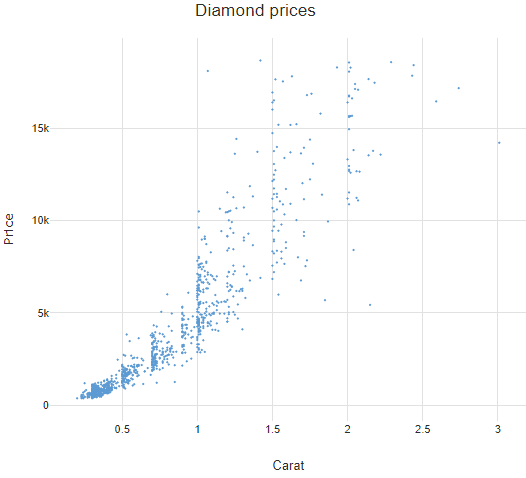
\includegraphics{DiamondPrices}
	\end{center}

\end{frame}		

\begin{frame}
	\frametitle{\insertsection} 
	\framesubtitle{\insertsubsection} 
	
	\begin{center}
		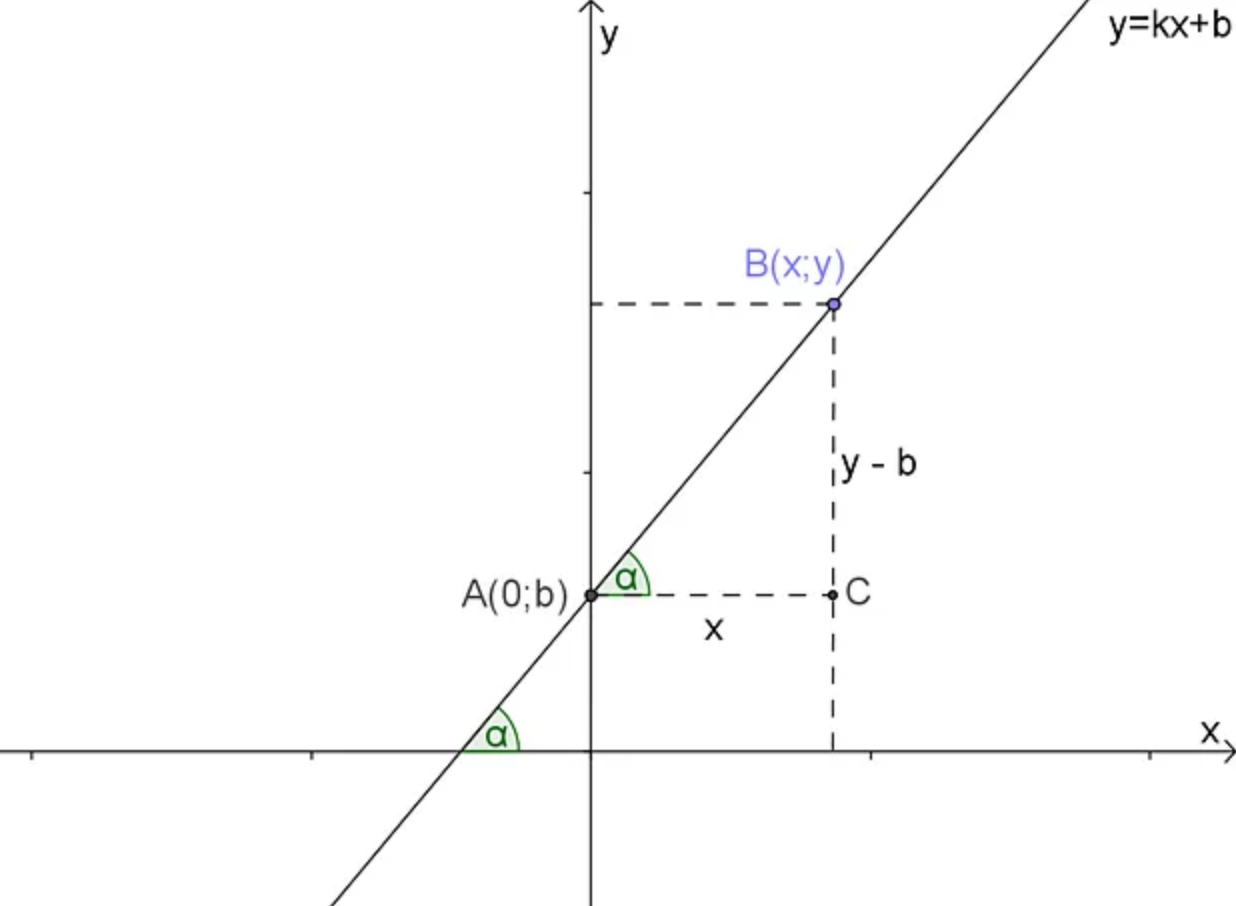
\includegraphics[scale=0.3]{lin1}
	\end{center}
	
\end{frame}	

\begin{frame}
	\frametitle{\insertsection} 
	\framesubtitle{\insertsubsection} 
	What if we have smth like this?
	\begin{center}
		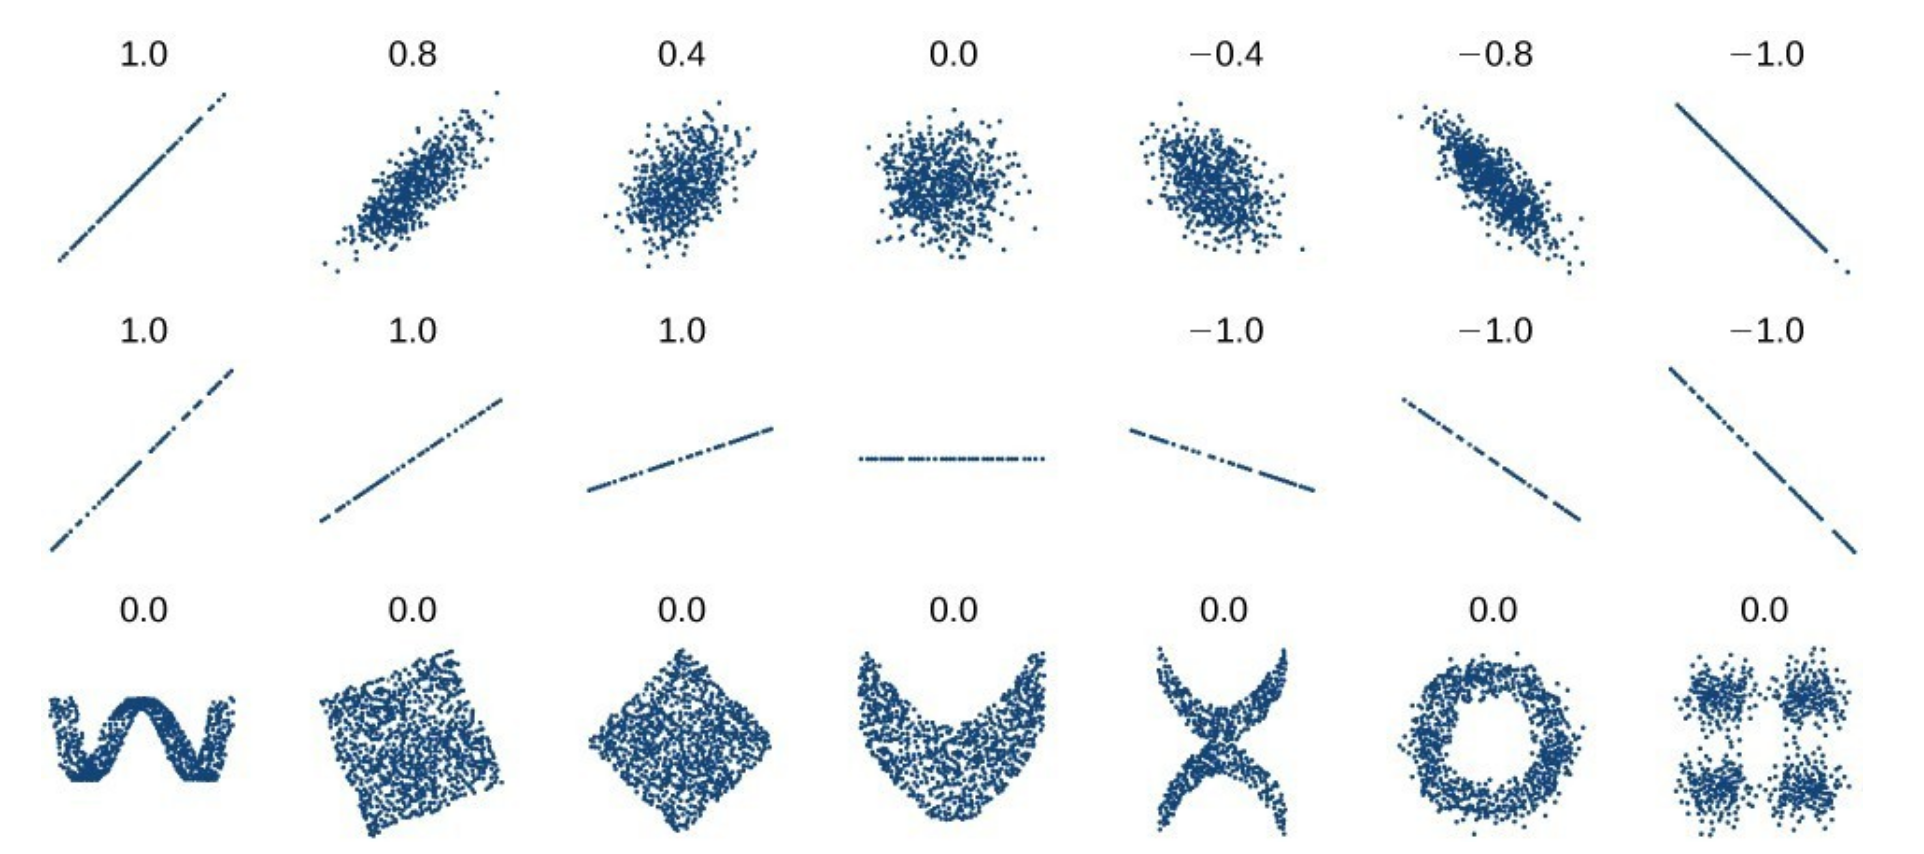
\includegraphics[scale=0.3]{nonlin1}
	\end{center}
	
\end{frame}	

\begin{frame}
	\frametitle{\insertsection} 
	\framesubtitle{\insertsubsection} 
	
	Once we decided that our data can be fitted by line model, let's select $\beta$ coefs. Let's follow \href{http://jalammar.github.io/visual-interactive-guide-basics-neural-networks/}{here}.
	
\end{frame}	

\section{Estimators}

\begin{frame}
	\frametitle{\insertsection} 
	\framesubtitle{\insertsubsection} 
	Estimation method (aka LOSS functions) - equation that help to find coefs. The most common techniques:
	\begin{itemize}
		\item OLS: $\beta = \Sigma(\hat{y} - y)^2 \rightarrow min$
		\item MLE: $\theta = P(X|\theta) \rightarrow max$
		\item Other purpose specified (Ridge, Quantile, PLS, Bayes Models)
		\end{itemize}
	
\end{frame}	



\subsection{When and what}

\begin{frame}
	\frametitle{\insertsection} 
	\framesubtitle{\insertsubsection} 
	What should I use for my model?
	\begin{itemize}
		\item OLS (and ols related): only continious variables
		\item MLE (and lme related): all other varaibles ()
		\item MCMC (and MC ralated): Bayes modeling 
	\end{itemize}
	
\end{frame}	

\section{How it works inside}
	
\begin{frame}
	\frametitle{\insertsection} 
	\framesubtitle{\insertsubsection} 
	
	
\end{frame}	


\end{document} 